% Options for packages loaded elsewhere
\PassOptionsToPackage{unicode}{hyperref}
\PassOptionsToPackage{hyphens}{url}
%
\documentclass[
]{book}
\usepackage{amsmath,amssymb}
\usepackage{lmodern}
\usepackage{iftex}
\ifPDFTeX
  \usepackage[T1]{fontenc}
  \usepackage[utf8]{inputenc}
  \usepackage{textcomp} % provide euro and other symbols
\else % if luatex or xetex
  \usepackage{unicode-math}
  \defaultfontfeatures{Scale=MatchLowercase}
  \defaultfontfeatures[\rmfamily]{Ligatures=TeX,Scale=1}
\fi
% Use upquote if available, for straight quotes in verbatim environments
\IfFileExists{upquote.sty}{\usepackage{upquote}}{}
\IfFileExists{microtype.sty}{% use microtype if available
  \usepackage[]{microtype}
  \UseMicrotypeSet[protrusion]{basicmath} % disable protrusion for tt fonts
}{}
\makeatletter
\@ifundefined{KOMAClassName}{% if non-KOMA class
  \IfFileExists{parskip.sty}{%
    \usepackage{parskip}
  }{% else
    \setlength{\parindent}{0pt}
    \setlength{\parskip}{6pt plus 2pt minus 1pt}}
}{% if KOMA class
  \KOMAoptions{parskip=half}}
\makeatother
\usepackage{xcolor}
\usepackage{color}
\usepackage{fancyvrb}
\newcommand{\VerbBar}{|}
\newcommand{\VERB}{\Verb[commandchars=\\\{\}]}
\DefineVerbatimEnvironment{Highlighting}{Verbatim}{commandchars=\\\{\}}
% Add ',fontsize=\small' for more characters per line
\usepackage{framed}
\definecolor{shadecolor}{RGB}{248,248,248}
\newenvironment{Shaded}{\begin{snugshade}}{\end{snugshade}}
\newcommand{\AlertTok}[1]{\textcolor[rgb]{0.94,0.16,0.16}{#1}}
\newcommand{\AnnotationTok}[1]{\textcolor[rgb]{0.56,0.35,0.01}{\textbf{\textit{#1}}}}
\newcommand{\AttributeTok}[1]{\textcolor[rgb]{0.77,0.63,0.00}{#1}}
\newcommand{\BaseNTok}[1]{\textcolor[rgb]{0.00,0.00,0.81}{#1}}
\newcommand{\BuiltInTok}[1]{#1}
\newcommand{\CharTok}[1]{\textcolor[rgb]{0.31,0.60,0.02}{#1}}
\newcommand{\CommentTok}[1]{\textcolor[rgb]{0.56,0.35,0.01}{\textit{#1}}}
\newcommand{\CommentVarTok}[1]{\textcolor[rgb]{0.56,0.35,0.01}{\textbf{\textit{#1}}}}
\newcommand{\ConstantTok}[1]{\textcolor[rgb]{0.00,0.00,0.00}{#1}}
\newcommand{\ControlFlowTok}[1]{\textcolor[rgb]{0.13,0.29,0.53}{\textbf{#1}}}
\newcommand{\DataTypeTok}[1]{\textcolor[rgb]{0.13,0.29,0.53}{#1}}
\newcommand{\DecValTok}[1]{\textcolor[rgb]{0.00,0.00,0.81}{#1}}
\newcommand{\DocumentationTok}[1]{\textcolor[rgb]{0.56,0.35,0.01}{\textbf{\textit{#1}}}}
\newcommand{\ErrorTok}[1]{\textcolor[rgb]{0.64,0.00,0.00}{\textbf{#1}}}
\newcommand{\ExtensionTok}[1]{#1}
\newcommand{\FloatTok}[1]{\textcolor[rgb]{0.00,0.00,0.81}{#1}}
\newcommand{\FunctionTok}[1]{\textcolor[rgb]{0.00,0.00,0.00}{#1}}
\newcommand{\ImportTok}[1]{#1}
\newcommand{\InformationTok}[1]{\textcolor[rgb]{0.56,0.35,0.01}{\textbf{\textit{#1}}}}
\newcommand{\KeywordTok}[1]{\textcolor[rgb]{0.13,0.29,0.53}{\textbf{#1}}}
\newcommand{\NormalTok}[1]{#1}
\newcommand{\OperatorTok}[1]{\textcolor[rgb]{0.81,0.36,0.00}{\textbf{#1}}}
\newcommand{\OtherTok}[1]{\textcolor[rgb]{0.56,0.35,0.01}{#1}}
\newcommand{\PreprocessorTok}[1]{\textcolor[rgb]{0.56,0.35,0.01}{\textit{#1}}}
\newcommand{\RegionMarkerTok}[1]{#1}
\newcommand{\SpecialCharTok}[1]{\textcolor[rgb]{0.00,0.00,0.00}{#1}}
\newcommand{\SpecialStringTok}[1]{\textcolor[rgb]{0.31,0.60,0.02}{#1}}
\newcommand{\StringTok}[1]{\textcolor[rgb]{0.31,0.60,0.02}{#1}}
\newcommand{\VariableTok}[1]{\textcolor[rgb]{0.00,0.00,0.00}{#1}}
\newcommand{\VerbatimStringTok}[1]{\textcolor[rgb]{0.31,0.60,0.02}{#1}}
\newcommand{\WarningTok}[1]{\textcolor[rgb]{0.56,0.35,0.01}{\textbf{\textit{#1}}}}
\usepackage{longtable,booktabs,array}
\usepackage{calc} % for calculating minipage widths
% Correct order of tables after \paragraph or \subparagraph
\usepackage{etoolbox}
\makeatletter
\patchcmd\longtable{\par}{\if@noskipsec\mbox{}\fi\par}{}{}
\makeatother
% Allow footnotes in longtable head/foot
\IfFileExists{footnotehyper.sty}{\usepackage{footnotehyper}}{\usepackage{footnote}}
\makesavenoteenv{longtable}
\usepackage{graphicx}
\makeatletter
\def\maxwidth{\ifdim\Gin@nat@width>\linewidth\linewidth\else\Gin@nat@width\fi}
\def\maxheight{\ifdim\Gin@nat@height>\textheight\textheight\else\Gin@nat@height\fi}
\makeatother
% Scale images if necessary, so that they will not overflow the page
% margins by default, and it is still possible to overwrite the defaults
% using explicit options in \includegraphics[width, height, ...]{}
\setkeys{Gin}{width=\maxwidth,height=\maxheight,keepaspectratio}
% Set default figure placement to htbp
\makeatletter
\def\fps@figure{htbp}
\makeatother
\setlength{\emergencystretch}{3em} % prevent overfull lines
\providecommand{\tightlist}{%
  \setlength{\itemsep}{0pt}\setlength{\parskip}{0pt}}
\setcounter{secnumdepth}{5}
\usepackage{booktabs}
\usepackage{amsthm}
\makeatletter
\def\thm@space@setup{%
  \thm@preskip=8pt plus 2pt minus 4pt
  \thm@postskip=\thm@preskip
}
\makeatother
\ifLuaTeX
  \usepackage{selnolig}  % disable illegal ligatures
\fi
\usepackage[]{natbib}
\bibliographystyle{plainnat}
\IfFileExists{bookmark.sty}{\usepackage{bookmark}}{\usepackage{hyperref}}
\IfFileExists{xurl.sty}{\usepackage{xurl}}{} % add URL line breaks if available
\urlstyle{same} % disable monospaced font for URLs
\hypersetup{
  pdftitle={GEOG0030: Geocomputation},
  pdfauthor={Justin van Dijk},
  hidelinks,
  pdfcreator={LaTeX via pandoc}}

\title{GEOG0030: Geocomputation}
\author{Justin van Dijk}
\date{Last modified: 2022-11-25}

\begin{document}
\maketitle

{
\setcounter{tocdepth}{1}
\tableofcontents
}
\hypertarget{module-overview}{%
\chapter*{Module Overview}\label{module-overview}}
\addcontentsline{toc}{chapter}{Module Overview}

\hypertarget{module-introduction}{%
\chapter*{Module Introduction}\label{module-introduction}}
\addcontentsline{toc}{chapter}{Module Introduction}

\begin{center}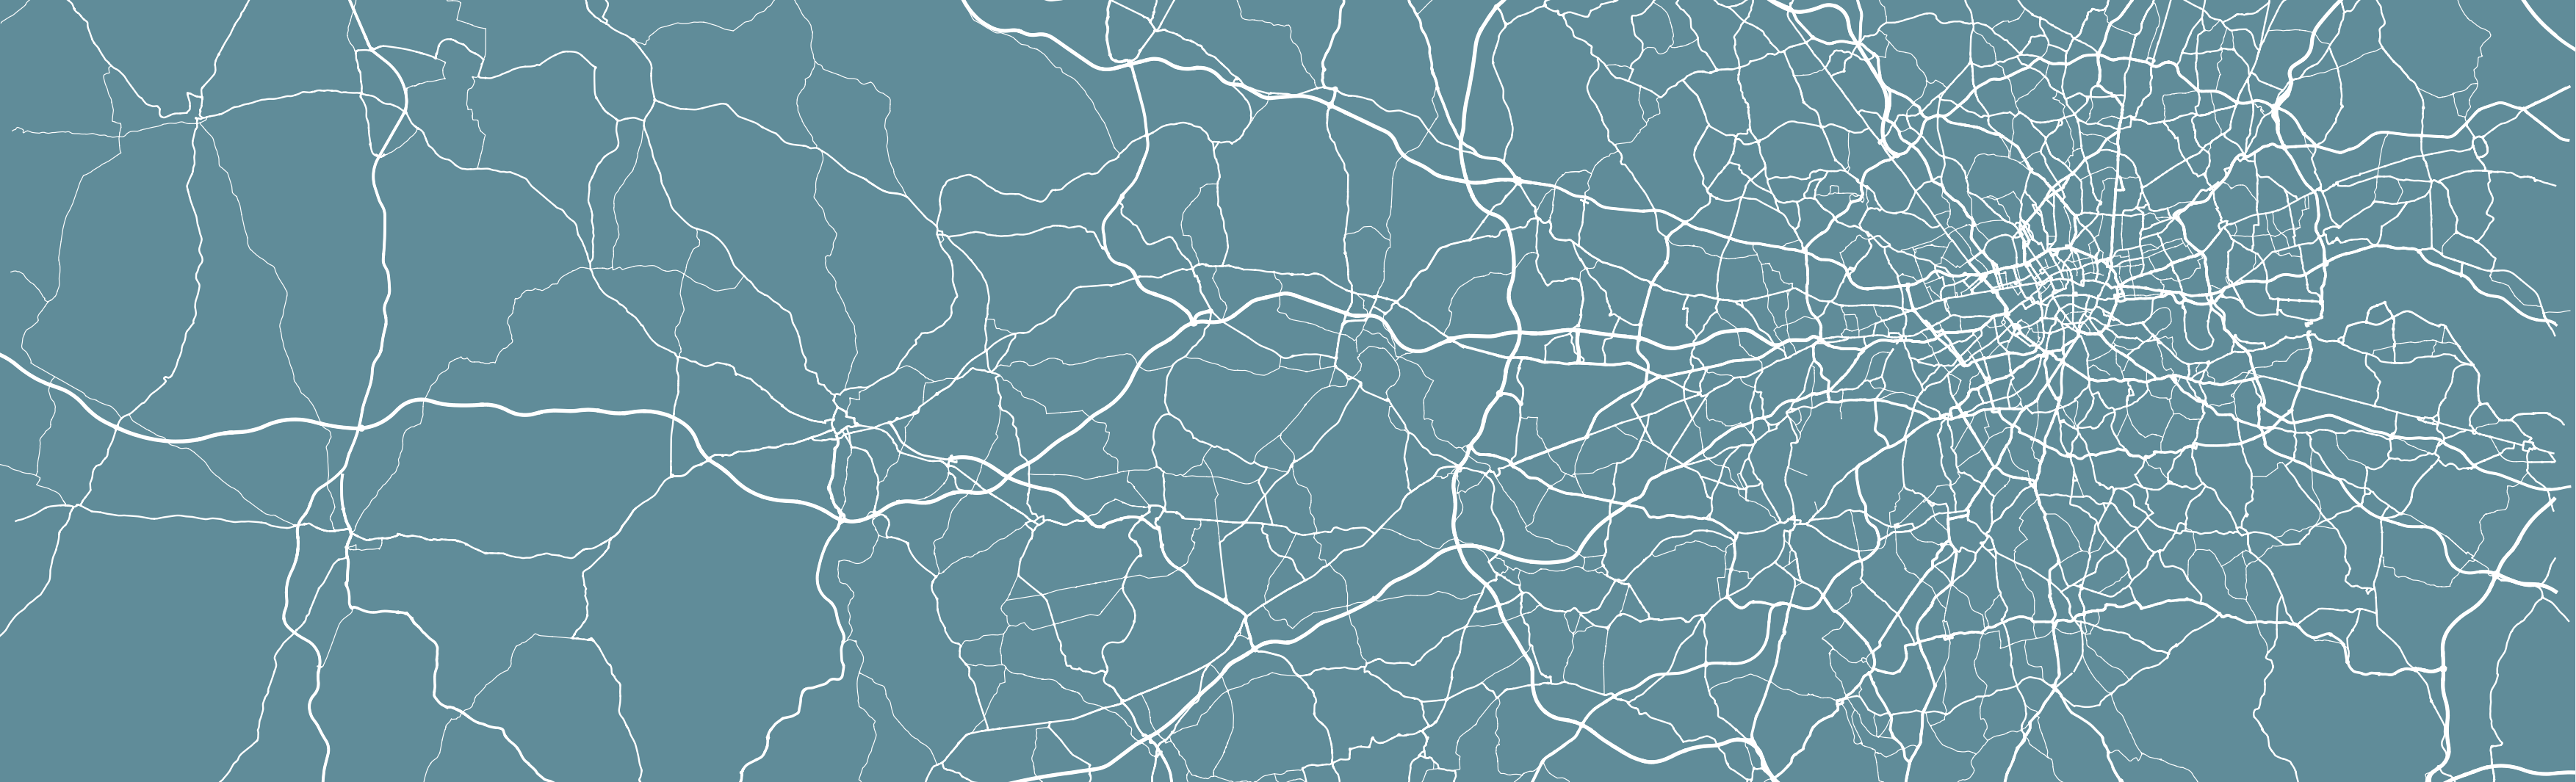
\includegraphics[width=1\linewidth]{images/general/geocomputation_welcome} \end{center}

\hypertarget{welcome}{%
\section*{Welcome}\label{welcome}}
\addcontentsline{toc}{section}{Welcome}

Welcome to \textbf{Geocomputation}. This module will introduce you both to the principles of spatial analysis as well as provide you with a comprehensive introduction to the use of programming. Over the next ten weeks, you will learn about the theory, methods and tools of spatial analysis through relevant case studies. We will start by using QGIS before moving to the R programming language. You will learn how to find, manage and clean spatial, demographic and socioeconomic datasets, and then analyse them using core spatial and statistical analysis techniques.

\hypertarget{moodle}{%
\section*{Moodle}\label{moodle}}
\addcontentsline{toc}{section}{Moodle}

\href{https://moodle.ucl.ac.uk/}{Moodle} is the central point of contact for GEOG0030 and it is where all important information will be communicated such as key module and assessment information. This workbook contains links to all reading material as well as the content of all computer tutorials

\hypertarget{module-overview-1}{%
\section*{Module overview}\label{module-overview-1}}
\addcontentsline{toc}{section}{Module overview}

The topics covered over the next ten weeks are:

\begin{longtable}[]{@{}
  >{\raggedright\arraybackslash}p{(\columnwidth - 4\tabcolsep) * \real{0.1212}}
  >{\raggedright\arraybackslash}p{(\columnwidth - 4\tabcolsep) * \real{0.3030}}
  >{\raggedright\arraybackslash}p{(\columnwidth - 4\tabcolsep) * \real{0.5758}}@{}}
\toprule()
\begin{minipage}[b]{\linewidth}\raggedright
Week
\end{minipage} & \begin{minipage}[b]{\linewidth}\raggedright
Section
\end{minipage} & \begin{minipage}[b]{\linewidth}\raggedright
Topic
\end{minipage} \\
\midrule()
\endhead
1 & Foundational Concepts & \href{geocomputation-an-introduction.html}{Geocomputation: An Introduction} \\
2 & Foundational Concepts & \href{giscience-and-gis-software.html}{GIScience and GIS software} \\
3 & Foundational Concepts & \href{cartography-and-visualisation.html}{Cartography and Visualisation} \\
4 & Foundational Concepts & \href{programming-for-data-analysis.html}{Programming for Data Analysis} \\
5 & Foundational Concepts & \href{programming-for-spatial-analysis.html}{Programming for Spatial Analysis} \\
& \textbf{Reading week} & \textbf{Reading week} \\
6 & Core Spatial Analysis & \href{analysing-spatial-patterns-i-geometric-operations-and-spatial-queries.html}{Analysing Spatial Patterns I: Geometric Operations and Spatial Queries} \\
7 & Core Spatial Analysis & \href{analysing-spatial-patterns-ii-spatial-autocorrelation.html}{Analysing Spatial Patterns II: Spatial Autocorrelation} \\
8 & Core Spatial Analysis & \href{analysing-spatial-patterns-iii-point-pattern-analysis.html}{Analysing Spatial Patterns III: Point Pattern Analysis} \\
9 & Advanced Spatial Analysis & \href{rasters-zonal-statistics-and-interpolation.html}{Rasters, Zonal Statistics and Interpolation} \\
10 & Advanced Spatial Analysis & \href{transport-network-analysis.html}{Transport Network Analysis} \\
\bottomrule()
\end{longtable}

\hypertarget{troubleshooting}{%
\section*{Troubleshooting}\label{troubleshooting}}
\addcontentsline{toc}{section}{Troubleshooting}

Spatial analysis can yield fascinating insights into geographical relationships, albeit at times it can be challenging, particularly when we combine this with learning how to program at the same time. You will most likely encounter many error messages, experience software crashes, and spend hours to identify bugs in your code. However, the rewards of learning how to programmatically solve complex spatial problems will be very much worth it in the end.

If you need specific assistance with this course please:

\begin{itemize}
\tightlist
\item
  Ask a question at the end of a lecture or during the computer practical.
\item
  Attend the Department's \textbf{Coding Therapy sessions} that are run on a weekly basis.
\item
  Check the \href{https://moodle.ucl.ac.uk/}{Moodle} assessment tab for queries relating to this module's assessment.
\end{itemize}

If after pursuing all these avenues you still need help, you can book into our office hours. You can use an office hour to discuss a geographical concept in relation to the material, assessment or for any personal matters relevant to the completion of the module.

\hypertarget{acknowledgements}{%
\section*{Acknowledgements}\label{acknowledgements}}
\addcontentsline{toc}{section}{Acknowledgements}

This year's workbook is updated and compiled using:

\begin{itemize}
\tightlist
\item
  The \href{https://jo-wilkin.github.io/GEOG0030/coursebook/index.html}{GEOG0030: Geocomputation 2021-2021} workbook as created and compiled by Dr Jo Wilkin.
\item
  The \href{https://jtvandijk.github.io/GEOG0030_20212022/}{GEOG0030: Geocomputation 2021-2022} workbook.
\end{itemize}

The datasets used in this workbook contain:

\begin{itemize}
\tightlist
\item
  Crime data obtained from \href{https://data.police.uk/}{data.police.uk} (Open Government Licence)
\item
  National Statistics data © Crown copyright and database right {[}2015{]} (Open Government Licence)
\item
  Ordnance Survey data © Crown copyright and database right {[}2015{]}
\item
  Public Health England © Crown copyright 2021
\end{itemize}

\hypertarget{foundational-concepts}{%
\chapter*{Foundational Concepts}\label{foundational-concepts}}
\addcontentsline{toc}{chapter}{Foundational Concepts}

\hypertarget{geocomputation-an-introduction}{%
\chapter{Geocomputation: An Introduction}\label{geocomputation-an-introduction}}

This week's lecture provided you with a thorough introduction on Geocomputation, outlining how and why it is different to a traditional GIScience course. We set the scene for the remainder of the module and explained how the foundational concepts that you will learn in the first half of term sit within the overall module. This week we start easy by setting up our work environment and set up the software that we will need over the coming weeks.

\hypertarget{reading-w01}{%
\section{Reading list}\label{reading-w01}}

\hypertarget{essential-readings}{%
\subsubsection*{Essential readings}\label{essential-readings}}
\addcontentsline{toc}{subsubsection}{Essential readings}

\begin{itemize}
\tightlist
\item
  Brundson, C. and Comber, A. 2020. Opening practice: Supporting reproducibility and critical spatial data science. \emph{Journal of Geographical Systems} 23: 477--496. \href{https://doi.org/10.1007/s10109-020-00334-2}{{[}Link{]}}
\item
  Longley, P. \emph{et al.} 2015. Geographic Information Science \& Systems, \textbf{Chapter 1}: \emph{Geographic Information: Science, Systems, and Society}. \href{https://ucl.rl.talis.com/link?url=https\%3A\%2F\%2Fapp.knovel.com\%2Fhotlink\%2Ftoc\%2Fid\%3AkpGISSE001\%2Fgeographic-information-science\%3Fkpromoter\%3Dmarc\&sig=e437927b963cc591dcb65491eccdd3869cc31aef80e1443cb2ba12d8f3bb031a}{{[}Link{]}}
\item
  Singleton, A. and Arribas-Bel, D. 2019. Geographic Data Science. \emph{Geographical Analysis}. \href{https://doi.org/10.1111/gean.12194}{{[}Link{]}}
\end{itemize}

\hypertarget{suggested-readings}{%
\subsubsection*{Suggested readings}\label{suggested-readings}}
\addcontentsline{toc}{subsubsection}{Suggested readings}

\begin{itemize}
\tightlist
\item
  Miller, H. and Goodchild, M. 2015. Data-driven geography. \emph{GeoJournal} 80: 449--461. \href{https://doi.org/10.1007/s10708-014-9602-6}{{[}Link{]}}
\item
  Goodchild, M. 2009. Geographic information systems and science: Today and tomorrow. \emph{Annals of GIS} 15(1): 3-9. \href{https://doi.org/10.1080/19475680903250715}{{[}Link{]}}
\end{itemize}

\hypertarget{getting-started}{%
\section{Getting started}\label{getting-started}}

Over the next few weeks, we will be taking a closer look at many of the foundational concepts that will ultimately enable you to confidently and competently analyse spatial data using both programming and GIS software. You will further learn how to plan, structure and conduct your own spatial analysis using programming -- whilst making decisions on how to best present your work, which is a crucial aspect of any type of investigation but of particular relevance to your dissertation.

To help with this, we highly recommend that you try to stay organised with your work, including taking notes and making yourself a coding handbook. We would also suggest to list the different datasets you come across - and importantly, the scales and different projections you use them at - more on this over the next weeks. Finally, you should also make notes about the different spatial analysis techniques you come across, including the different properties they assess and parameters they require to run.

\hypertarget{software}{%
\section{Software}\label{software}}

This course primarily uses the \href{https://www.r-project.org/}{R} programming language, although we start by using \href{https://qgis.org/en/site/}{QGIS} in the next two weeks to give you a basic foundation in the principles of spatial analysis.

\textbf{Note}
Please follow the instructions below to install both \href{https://www.r-project.org/}{R} and \href{https://qgis.org/en/site/}{QGIS} onto your own personal computer. If you cannot install the software on your personal computer or you are not planning to bring your own laptop to the computer practicals, please refer to the \protect\hyperlink{ucl}{UCL Desktop and RStudio Server} section below. Please make sure that you have access to a working installation of QGIS and R (including relevant packages) \textbf{before} the first hands-on practical session next week.

\hypertarget{qgis-installation}{%
\subsection{QGIS Installation}\label{qgis-installation}}

QGIS is an open-source graphic user interface GIS with many community developed add-on packages (or plugins) that provide additional functionality to the software. You can download and install QGIS on your personal machine by going to the QGIS website: \href{https://qgis.org/en/site/forusers/download.html}{{[}Link{]}}.

\textbf{Note}
We recommend installing the \textbf{Long Term Release} (\emph{QGIS 3.22 LTR}) as this version should be the most stable version. For Windows users: the QGIS installation may be a little slow.

After installation, start QGIS to see if the installation was successful and no errors are shown after start up.

\hypertarget{r-and-rstudio-installation}{%
\subsection{R and RStudio Installation}\label{r-and-rstudio-installation}}

R is both a programming language and software environment - in the form of RStudio- originally designed for statistical computing and graphics. R's great strength is that it is open-source, can be used on any computer operating system, and is free for anyone to use and contribute to. Because of this, it is rapidly becoming the statistical language of choice for many academics and has a very large user community with people constantly contributing new packages to carry out all manner of statistical, graphical, and importantly for us, geographical tasks.

Installing R takes a few relatively simple steps involving two programmes. First there is the R programme itself. Follow these steps to get it installed on your computer:

\begin{enumerate}
\def\labelenumi{\arabic{enumi}.}
\tightlist
\item
  Navigate in your browser to your nearest CRAN mirror: \href{https://cran.ma.imperial.ac.uk/}{{[}Link{]}}
\item
  If you use a Windows computer, click on \emph{Download R for Windows}. Then click on \emph{base}. Download and install \textbf{R 4.2.x for Windows}. If you use a Mac computer, click on \emph{Download R for macOS} and download and install \textbf{R-4.2.x.pkg}
\end{enumerate}

That is it! You now have installed the latest version of R on your own machine. However, to make working with R a little bit easier we also need to install something called an Integrated Development Environment (IDE). We will use RStudio:

\begin{enumerate}
\def\labelenumi{\arabic{enumi}.}
\tightlist
\item
  Navigate to the official webpage of RStudio: \href{https://posit.co/download/rstudio-desktop/\#download}{{[}Link{]}}
\item
  Download and install RStudio Desktop on your computer (\textbf{free version!})
\end{enumerate}

After this, start RStudio to see if the installation was successful and no errors are shown after start up.

\hypertarget{ucl}{%
\subsection{UCL Desktop and RStudio Server}\label{ucl}}

As an alternative to installing QGIS and R with RStudio onto your personal device, there are some other options. Firstly, both programmes are available through \href{https://www.ucl.ac.uk/isd/services/computers/remote-access/desktopucl-anywhere}{Desktop@UCL Anywhere} as well as all UCL computers on campus. In case of R, there is also an RStudio server version available which you can access through your web browser: \href{https://rstudio.data-science.rc.ucl.ac.uk/}{{[}Link{]}}

You should be able to log in with your normal UCL username and password. After logging in, you should see the RStudio interface appear.

\begin{figure}

{\centering 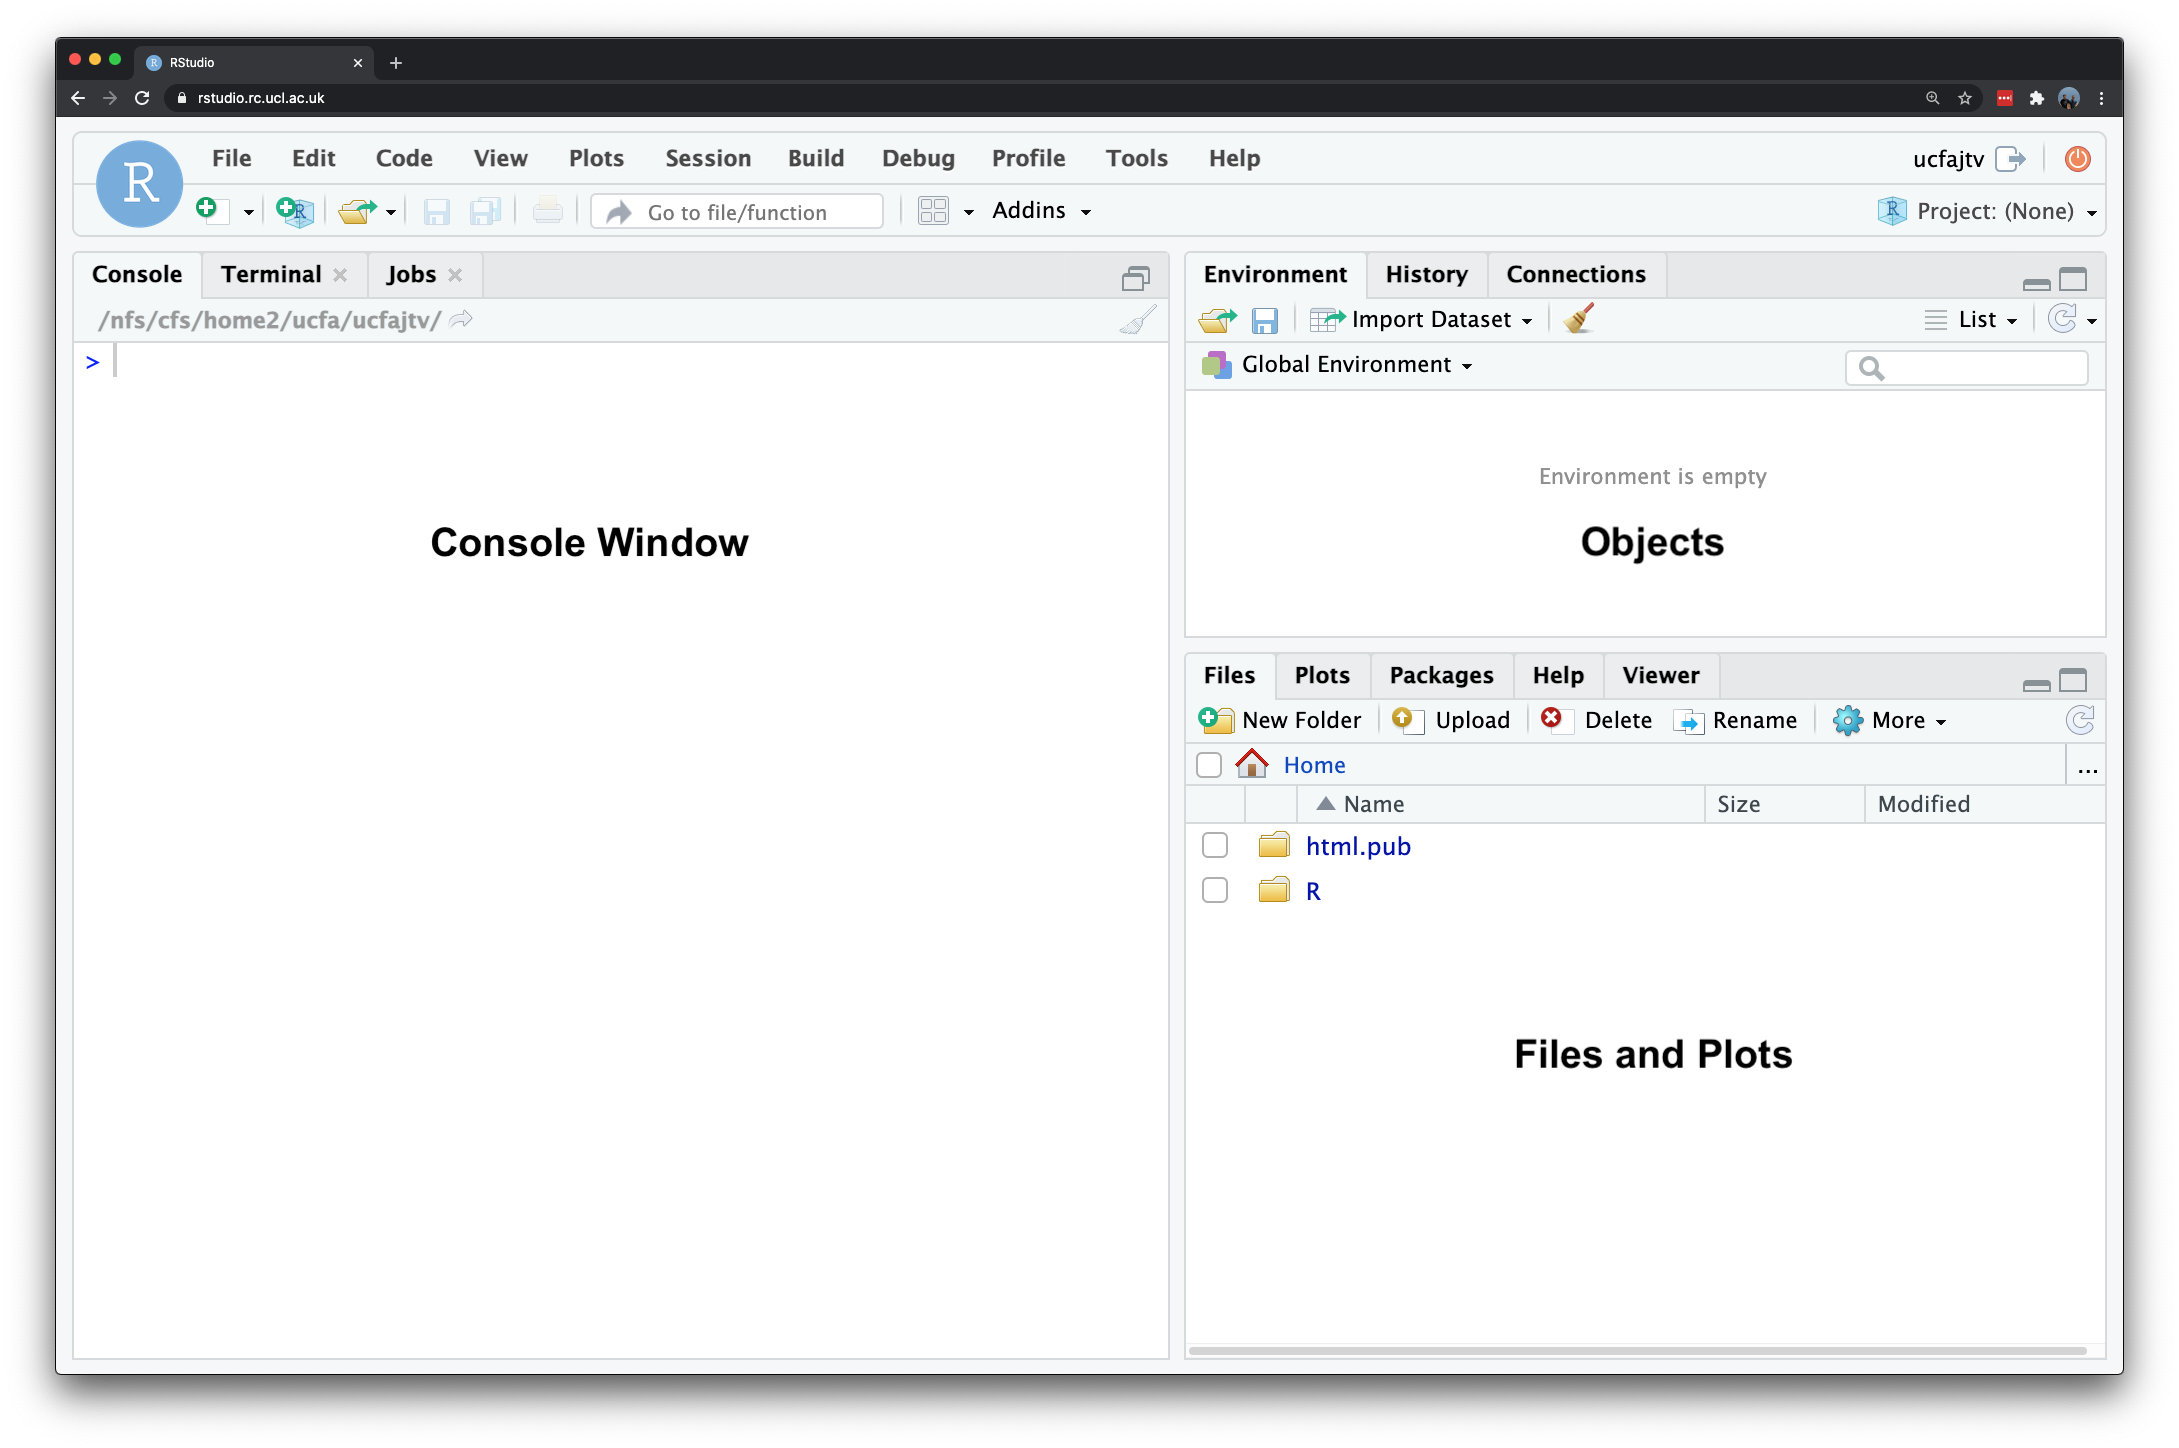
\includegraphics[width=30.26in]{images/w01/rstudio_interface} 

}

\caption{The RStudio Server interface.}\label{fig:01-rstudio-interface}
\end{figure}

\textbf{Note}
If it is the first time you log on to RStudio server you may only see the RStudio interface appear once you have clicked on the \emph{start a new session} button. More importantly: if you are not on campus, RStudio server will only work with an active Virtual Private Network (VPN) connection that links your personal computer into UCL's network. Details on setting up a VPN connection can be found in UCL's VPN connection guides: \href{https://www.ucl.ac.uk/isd/services/get-connected/ucl-virtual-private-network-vpn}{{[}Link{]}}

\hypertarget{r-package-installation}{%
\subsection{R package installation}\label{r-package-installation}}

Now we have installed or have access to QGIS and R, we need to customise R. Many useful R function come in packages, these are free libraries of code written and made available by other by R users. This includes packages specifically developed for data cleaning, data wrangling, visualisation, mapping, and spatial analysis. To save us some time, we will install all R packages that we will need over the next ten weeks in one go. Without going into detail on the RStudio (Server) interface, copy and paste the following code into the \textbf{console}. You can execute the code by hitting \textbf{Enter}. This may take a while.

\begin{Shaded}
\begin{Highlighting}[]
\CommentTok{\# install all packages that we need}
\FunctionTok{install.packages}\NormalTok{(}\FunctionTok{c}\NormalTok{(}\StringTok{"tidyverse"}\NormalTok{, }\StringTok{"sf"}\NormalTok{, }\StringTok{"tmap"}\NormalTok{, }\StringTok{"osmdata"}\NormalTok{, }\StringTok{"RColorBrewer"}\NormalTok{, }\StringTok{"janitor"}\NormalTok{,}
    \StringTok{"spdep"}\NormalTok{, }\StringTok{"dbscan"}\NormalTok{, }\StringTok{"raster"}\NormalTok{, }\StringTok{"spatstat"}\NormalTok{, }\StringTok{"gstat"}\NormalTok{, }\StringTok{"dodgr"}\NormalTok{))}
\end{Highlighting}
\end{Shaded}

Once you have installed the packages, we need to check whether we can in fact load them into our R session. Copy and paste the following code into the \textbf{console}, and executed by hitting \textbf{Enter} again.

\begin{Shaded}
\begin{Highlighting}[]
\CommentTok{\# load all packages}
\FunctionTok{library}\NormalTok{(tidyverse)}
\end{Highlighting}
\end{Shaded}

\begin{verbatim}
## -- Attaching packages ----------------------------------------------------------------------------------- tidyverse 1.3.2 --
## v ggplot2 3.4.0      v purrr   0.3.5 
## v tibble  3.1.8      v dplyr   1.0.10
## v tidyr   1.2.1      v stringr 1.4.1 
## v readr   2.1.3      v forcats 0.5.2 
## -- Conflicts -------------------------------------------------------------------------------------- tidyverse_conflicts() --
## x dplyr::filter() masks stats::filter()
## x dplyr::lag()    masks stats::lag()
\end{verbatim}

\begin{Shaded}
\begin{Highlighting}[]
\FunctionTok{library}\NormalTok{(sf)}
\end{Highlighting}
\end{Shaded}

\begin{verbatim}
## Linking to GEOS 3.10.2, GDAL 3.4.2, PROJ 8.2.1; sf_use_s2() is TRUE
\end{verbatim}

\begin{Shaded}
\begin{Highlighting}[]
\FunctionTok{library}\NormalTok{(tmap)}
\FunctionTok{library}\NormalTok{(osmdata)}
\end{Highlighting}
\end{Shaded}

\begin{verbatim}
## Data (c) OpenStreetMap contributors, ODbL 1.0. https://www.openstreetmap.org/copyright
\end{verbatim}

\begin{Shaded}
\begin{Highlighting}[]
\FunctionTok{library}\NormalTok{(RColorBrewer)}
\FunctionTok{library}\NormalTok{(janitor)}
\end{Highlighting}
\end{Shaded}

\begin{verbatim}
## 
## Attaching package: 'janitor'
## 
## The following objects are masked from 'package:stats':
## 
##     chisq.test, fisher.test
\end{verbatim}

\begin{Shaded}
\begin{Highlighting}[]
\FunctionTok{library}\NormalTok{(spdep)}
\end{Highlighting}
\end{Shaded}

\begin{verbatim}
## Loading required package: sp
## Loading required package: spData
## To access larger datasets in this package, install the spDataLarge
## package with: `install.packages('spDataLarge',
## repos='https://nowosad.github.io/drat/', type='source')`
\end{verbatim}

\begin{Shaded}
\begin{Highlighting}[]
\FunctionTok{library}\NormalTok{(dbscan)}
\end{Highlighting}
\end{Shaded}

\begin{verbatim}
## 
## Attaching package: 'dbscan'
## 
## The following object is masked from 'package:stats':
## 
##     as.dendrogram
\end{verbatim}

\begin{Shaded}
\begin{Highlighting}[]
\FunctionTok{library}\NormalTok{(raster)}
\end{Highlighting}
\end{Shaded}

\begin{verbatim}
## 
## Attaching package: 'raster'
## 
## The following object is masked from 'package:dplyr':
## 
##     select
\end{verbatim}

\begin{Shaded}
\begin{Highlighting}[]
\FunctionTok{library}\NormalTok{(spatstat)}
\end{Highlighting}
\end{Shaded}

\begin{verbatim}
## Loading required package: spatstat.data
## Loading required package: spatstat.geom
## spatstat.geom 3.0-3
## 
## Attaching package: 'spatstat.geom'
## 
## The following objects are masked from 'package:raster':
## 
##     area, rotate, shift
## 
## Loading required package: spatstat.random
## spatstat.random 3.0-1
## Loading required package: spatstat.explore
## Loading required package: nlme
## 
## Attaching package: 'nlme'
## 
## The following object is masked from 'package:raster':
## 
##     getData
## 
## The following object is masked from 'package:dplyr':
## 
##     collapse
## 
## spatstat.explore 3.0-5
## Loading required package: spatstat.model
## Loading required package: rpart
## spatstat.model 3.0-2
## Loading required package: spatstat.linnet
## spatstat.linnet 3.0-3
## 
## spatstat 3.0-2 
## For an introduction to spatstat, type 'beginner'
\end{verbatim}

\begin{Shaded}
\begin{Highlighting}[]
\FunctionTok{library}\NormalTok{(gstat)}
\end{Highlighting}
\end{Shaded}

\begin{verbatim}
## 
## Attaching package: 'gstat'
## 
## The following object is masked from 'package:spatstat.explore':
## 
##     idw
\end{verbatim}

\begin{Shaded}
\begin{Highlighting}[]
\FunctionTok{library}\NormalTok{(dodgr)}
\end{Highlighting}
\end{Shaded}

You will see some information printed to your console but as long as you do not get a message that is similar to \texttt{Error:\ package\ or\ namespace\ load\ failed\ for\ \textless{}packagename\textgreater{}} or \texttt{Error:\ package\ \textquotesingle{}\textless{}packagename\textquotesingle{}\ could\ not\ be\ loaded} all should be fine.

\textbf{Note}
Even if you have used R or RStudio Server before and already installed some of the packages in the above list, do re-install all packages to make sure you have the latest versions. Legacy installations that have not been updated may lay lead to problems when going through the tutorials.

\hypertarget{a-note-on-arcgis}{%
\subsection{A note on ArcGIS}\label{a-note-on-arcgis}}

\href{https://www.esri.com/en-us/arcgis/products/arcgis-pro/overview}{ArcGIS Pro} (previously ArcMap) is the main commercial GIS software that you may have already used - or seen/heard about through other modules or even job adverts. We do not use ArcGIS Pro in our Practicals for several reasons:

\begin{itemize}
\tightlist
\item
  Computing requirements for ArcGIS Pro are substantial and it \textbf{only} operates on the Windows Operating System. For Mac users, using ArcGIS Pro (and ArcMap) would require using either a Virtual Machine or running a copy of Windows OS on a separate partition of your hard drive.
\item
  It is \textbf{proprietary} software, which means you need a license to use the software. For those of us in education, the University covers the cost of this license, but when you leave, you will need to pay for a personal license (around £100 for non-commercial use) to continue using the software and repeat any analysis you have used the software for.
\item
  Whilst ArcPro can use pure \href{https://www.python.org/}{Python} (and even R) as a programming language within it through scripts and notebooks, it primarily relies on its own \textbf{ArcPy} and \textbf{ArcGIS API for Python} packages to run the in-built tools and analytical functions. To use these packages, you still need a license which makes it difficult to share your code with others \emph{if} they do not have their own ArcGIS license.
\end{itemize}

Recent developments in the ArcPro software, however, does make it an attractive tool for spatial data science and quantitative geography - it has cross-user functionality, from data analysts who like to use a tool called Notebooks for their code development, to those focused more on cartography and visualisation with in-built bridges to Adobe's Creative Suite. We therefore do not want to put you off looking into ArcGIS in the future, but for this course, we want to ensure the reproducibility of your work.

\textbf{Note} This also means that the analysis you will be doing for your coursework assignment must be completed in R and QGIS. Specific guidance on the coursework assignment and permitted software will be made available at the end of Reading Week.

\hypertarget{byl-w01}{%
\section{Before you leave}\label{byl-w01}}

You should now be all ready to go with the computer practicals the coming week. \href{https://www.youtube.com/watch?v=d8Fmu3RLEOY}{That is it for this week}!

\hypertarget{additional-resources}{%
\chapter*{Additional Resources}\label{additional-resources}}
\addcontentsline{toc}{chapter}{Additional Resources}

\hypertarget{data-sources}{%
\chapter{Data Sources}\label{data-sources}}

Below you will find a list of resources that you might want to explore when sourcing data for your coursework assignment or your dissertation. This is by no means an exhaustive list, but simply contains some suggestions of websites that you may want to use.

\textbf{Note}
You are \textbf{not limited} to using these datasets for your coursework assignment or your dissertation.

\hypertarget{open-data}{%
\section{Open Data}\label{open-data}}

The following websites contain Open Data or link to Open Data from several respectable data providers:

\begin{itemize}
\tightlist
\item
  \href{http://insideairbnb.com/get-the-data.html}{AirBnB Data}
\item
  \href{https://docs.ropensci.org/bikedata/}{Bike Docking Data (ready for R)}
\item
  \href{https://camdenairaction.wordpress.com/2017/02/20/schools-monitoring-project-spring-2017/}{Camden Air Action}
\item
  \href{https://data.cdrc.ac.uk/}{Consumer Data Research Centre}
\item
  \href{https://environment.data.gov.uk/}{DEFRA}
\item
  \href{https://www.diva-gis.org/}{DIVA-GIS}
\item
  \href{https://digimap.edina.ac.uk/}{Edina (e.g.~OS mastermap)}
\item
  \href{https://ec.europa.eu/eurostat/statistics-explained/index.php/Tourism_statistics}{EU Tourism Data}
\item
  \href{https://ec.europa.eu/eurostat}{Eurostat}
\item
  \href{https://www.geofabrik.de/}{Geofabrik (OSM data)}
\item
  \href{https://rp5.ru/Weather_in_the_world}{Global Weather Data}
\item
  \href{https://datasetsearch.research.google.com/}{Google Dataset Search}
\item
  \href{https://github.com/RamiKrispin/coronavirus}{Johns Hopkins COVID19 Data (ready for R}
\item
  \href{https://www.londonair.org.uk/LondonAir/Default.aspx}{King's College Data on Air Pollution}
\item
  \href{https://data.london.gov.uk/}{London Data Store}
\item
  \href{https://www.ft.com/content/6f381ad4-fef7-11e9-be59-e49b2a136b8d}{London Tube PM2.5 Levels}
\item
  \href{https://earthdata.nasa.gov/}{NASA EARTHDATA}
\item
  \href{https://sedac.ciesin.columbia.edu/}{NASA SocioEconomic Data and Applications Center (SEDAC)}
\item
  \href{https://nhs-r-community.github.io/NHSRdatasets/}{NHS Data (ready for R)}
\item
  \href{https://www.nomisweb.co.uk/}{nomis Official Census and Labour Market Statistics}
\item
  \href{https://geoportal.statistics.gov.uk/}{Office for National Statistics Geoportal}
\item
  \href{https://www.ons.gov.uk/}{Office for National Statistics}
\item
  \href{https://opentopography.org/}{Open Topography}
\item
  \href{https://www.nature.com/articles/s41597-020-0397-7}{Tesco Store Data (London)}
\item
  \href{https://cycling.data.tfl.gov.uk/}{TfL Cycling Data}
\item
  \href{https://tfl.gov.uk/info-for/open-data-users/our-open-data?intcmp=3671\#on-this-page-2}{TfL Open Data}
\item
  \href{https://github.com/rfordatascience/tidytuesday}{Tidy Tuesday Data (not exclusively spatial data)}
\item
  \href{https://movement.uber.com/?lang=en-GB}{Uber Travel Time Data}
\item
  \href{https://coronavirus.data.gov.uk/}{UK COVID19 Data}
\item
  \href{https://ukdataservice.ac.uk/}{UK Data Service}
\item
  \href{https://www.census.gov/data.html}{US Census Data}
\item
  \href{http://us-cities.survey.okfn.org/}{US City Open Data Census}
\item
  \href{https://earthexplorer.usgs.gov/}{USGS Earth Explorer}
\item
  \href{https://github.com/wpgp}{WorldPop GitHub}
\item
  \href{https://www.worldpop.org/}{WorldPop}
\end{itemize}

Some other websites that could be helpful:

\begin{itemize}
\tightlist
\item
  \href{https://github.com/awesomedata/awesome-public-datasets}{Awesome Public Datasets}; general collection of datasets, although not limited to spatial data.
\item
  \href{https://freegisdata.rtwilson.com/}{Free GIS data}; long list with lots of GIS datasets on many different topics and covering many different areas.
\end{itemize}

\hypertarget{safeguarded-data}{%
\section{Safeguarded Data}\label{safeguarded-data}}

Undergraduate students can also apply for a \textbf{Safeguarded} dataset held by the \href{https://www.cdrc.ac.uk/}{Consumer Data Research Centre}. There is a process to access these \textbf{Safeguarded} datasets, which is detailed on the \href{https://data.cdrc.ac.uk/using-our-data-services}{CDRC website}. Please be aware that it normally takes 4-5 weeks for your application to be processed.

As part of the process, you will need to say in your application why you want that specific dataset and what you are planning to do with it. You will also need to have at least thought about the ethical implications of using that data and provide this with your data application (alongside your standard ethics application).

Some of the datasets held by the CDRC that you can apply for are:

\begin{itemize}
\tightlist
\item
  \href{https://data.cdrc.ac.uk/dataset/bicycle-sharing-system-docking-station-observations}{Bicycle Sharing System Docking Station Observations}
\item
  \href{https://data.cdrc.ac.uk/dataset/cdrc-modelled-ethnicity-proportions-lsoa-geography}{CDRC Modelled Ethnicity Proportions - LSOA Geography}
\item
  \href{https://data.cdrc.ac.uk/dataset/fca-financial-lives-survey}{FCA Financial Lives Survey}
\item
  \href{https://data.cdrc.ac.uk/dataset/local-data-company-smartstreetsensor-footfall-data-\%E2\%80\%93-research-aggregated-data}{Local Data Company - SmartStreetSensor Footfall Data -- Research Aggregated data}
\item
  \href{https://data.cdrc.ac.uk/dataset/nhs-hospital-admission-rates-ethnic-group-and-other-characteristics}{NHS Hospital Admission Rates by Ethnic Group and other Characteristics}
\item
  \href{https://data.cdrc.ac.uk/dataset/speedchecker-broadband-internet-speed-tests}{Speedchecker Broadband Internet Speed Tests}
\end{itemize}

\textbf{Note}
Given that the application can take several weeks, the Safeguarded CDRC datasets may be useful for your dissertation work but probably not for the GEOG0030 coursework assignment. However, any of the CDRC datasets that are marked as \textbf{Open Data} do not require this application process and you can download these datasets directly after registering on the website.

\end{document}
